\documentclass[sigconf]{acmart}

\copyrightyear{2024}
\acmYear{2024}
\setcopyright{rightsretained}
\acmConference[WWW '24 Companion] {Companion Proceedings of the ACM Web Conference 2024}{May 13--17, 2024}{Singapore, Singapore.}
\acmBooktitle{Companion Proceedings of the ACM Web Conference 2024 (WWW '24 Companion), May 13--17, 2024, Singapore, Singapore}
\acmISBN{979-8-4007-0172-6/24/05}
\acmDOI{10.1145/XXXXXX.XXXXXX}
% 1 Authors, replace the red X's with your assigned DOI string during the rightsreview eform process.
% 2 Your DOI link will become active when the proceedings appears in the DL.
% 3 Retain the DOI string between the curly braces for uploading your presentation video.

\settopmatter{printacmref=true}

\usepackage[utf8]{inputenc}
\usepackage{graphicx}
\usepackage{enumitem}
\usepackage{float}
\usepackage[lofdepth,lotdepth]{subfig}
\def\subfloatautorefname{Subfigure}
\usepackage{listings}
\usepackage{color}
\definecolor{mediumgray}{rgb}{0.3, 0.4, 0.4}
\definecolor{mediumblue}{rgb}{0.0, 0.0, 0.8}
\definecolor{forestgreen}{rgb}{0.13, 0.55, 0.13}
\definecolor{darkviolet}{rgb}{0.58, 0.0, 0.83}
\definecolor{royalblue}{rgb}{0.25, 0.41, 0.88}
\definecolor{crimson}{rgb}{0.86, 0.8, 0.24}
\lstdefinelanguage{JavaScript}{
  morekeywords=[1]{break, continue, delete, else, for, function, if, in,
    new, return, this, typeof, var, void, while, with},
  % Literals, primitive types, and reference types.
  morekeywords=[2]{false, null, true, boolean, number, undefined,
    Array, Boolean, Date, Math, Number, String, Object},
  % Built-ins.
  morekeywords=[3]{eval, parseInt, parseFloat, escape, unescape},
  sensitive,
  morecomment=[s]{/*}{*/},
  morecomment=[l]//,
  morecomment=[s]{/**}{*/}, % JavaDoc style comments
  morestring=[b]',
    morestring=[b]`,
  morestring=[b]"
}[keywords, comments, strings]
\lstdefinelanguage[ECMAScript2015]{JavaScript}[]{JavaScript}{
  morekeywords=[1]{await, async, case, catch, class, const, default, do,
    enum, export, extends, finally, from, implements, import, instanceof,
    let, static, super, switch, throw, try},
  morestring=[b]` % Interpolation strings.
}
\lstdefinestyle{JSES6Base}{
  backgroundcolor=\color{white},
  basicstyle=\ttfamily,
  basicstyle=\small,
  breakatwhitespace=false,
  breaklines=false,
  captionpos=b,
  columns=fullflexible,
  commentstyle=\color{mediumgray}\upshape,
  emph={},
  emphstyle=\color{crimson},
  extendedchars=true,  % requires inputenc
  fontadjust=true,
  frame=single,
  identifierstyle=\color{black},
  keepspaces=true,
  keywordstyle=\color{mediumblue},
  keywordstyle={[2]\color{darkviolet}},
  keywordstyle={[3]\color{royalblue}},
  numbers=left,
  numbersep=5pt,
  numberstyle=\tiny\color{black},
  rulecolor=\color{black},
  showlines=true,
  showspaces=false,
  showstringspaces=false,
  showtabs=false,
  stringstyle=\color{forestgreen},
  tabsize=2,
  title=\lstname,
  upquote=true  % requires textcomp
}
\lstdefinestyle{JavaScript}{
  language=JavaScript,
  style=JSES6Base
}
\lstdefinestyle{ES6}{
  language=ES6,
  style=JSES6Base
}
\newlist{questions}{enumerate}{2}
\setlist[questions,1]{label=RQ\arabic*.,ref=RQ\arabic*}
\setlist[questions,2]{label=(\alph*),ref=\thequestionsi(\alph*)}

%%
%% end of the preamble, start of the body of the document source.
\begin{document}

%%
%% The "title" command has an optional parameter,
%% allowing the author to define a~"short title" to be used in page headers.
\title[Toward Making Opaque Web Content More Accessible]{Toward Making Opaque Web Content More Accessible: \protect\\ Accessibility From Adobe Flash to Canvas-Rendered Apps}

%%
%% The "author" command and its associated commands are used to define
%% the authors and their affiliations.
%% Of note is the shared affiliation of the first two authors, and the
%% "authornote" and "authornotemark" commands
%% used to denote shared contribution to the research.
\author{Thomas Steiner}
\orcid{0000-0001-7482-6129}
\email{tomac@google.com}
\affiliation{%  
  \institution{Google Germany GmbH}
  \streetaddress{ABC-Str. 19}
  \city{Hamburg}  
  \country{Germany}
  \postcode{20354}
}

%%
%% By default, the full list of authors will be used in the page
%% headers. Often, this list is too long, and will overlap
%% other information printed in the page headers. This command allows
%% the author to define a~more concise list
%% of authors' names for this purpose.
% \renewcommand{\shortauthors}{Trovato and Tobin, et al.}

%%
%% The abstract is a~short summary of the work to be presented in the
%% article.
\begin{abstract}
Adobe Flash, once a ubiquitous multimedia platform, played a pivotal role in shaping the digital landscape for nearly two decades. Its capabilities ranged from animated banners and immersive websites to complex online applications and games. Flash content was embedded on websites with the \texttt{embed} or the \texttt{object} element. To the browser, the embedded content is opaque by default, which means Flash content can't be used for the accessibility tree that the browser creates based on the \textsc{dom} tree, which is used by platform-specific accessibility \textsc{api}s to provide a representation that can be understood by assistive technologies, such as screen readers.

With Flash declining in popularity, \textsc{html}\ 5 introduced the \texttt{canvas} element, which for the first time allowed developers to draw graphics and animations with either the canvas scripting \textsc{api} or the Web\textsc{gl} \textsc{api} directly and natively in the browser. As with Flash, such canvas-rendered content is opaque by default and unusable for the accessibility tree. Ultimately, the implementation of the WebAssembly Garbage Collection (Wasm\textsc{gc}) standard in browsers allowed developers to port applications, written in non-Web programming languages like Kotlin for non-Web platforms like Android, to the Web by compiling them to Wasm\textsc{gc} and rendering the entire app into a \texttt{canvas}. In the most extreme of cases, this means that the entire \textsc{html} code of an application can consist of a sole \texttt{<canvas>} tag, which is opaque to the browser and impossible to read for the accessibility tree. Without judging their quality, this paper focuses on documenting approaches then and now for making such opaque Web content more accessible to users of assistive technologies.
\end{abstract}

%%
%% The code below is generated by the tool at http://dl.acm.org/ccs.cfm.
%% Please copy and paste the code instead of the example below.
%%
\begin{CCSXML}
<ccs2012>
<concept>
<concept_id>10002951.10003260.10003300.10003302</concept_id>
<concept_desc>Information systems~Browsers</concept_desc>
<concept_significance>500</concept_significance>
</concept>
</ccs2012>
\end{CCSXML}

\ccsdesc[500]{Information systems~Browsers}

%%
%% Keywords. The author(s) should pick words that accurately describe
%% the work being presented. Separate the keywords with commas.
\keywords{Adobe Flash, Canvas, WebAssembly, Wasm, Wasm\textsc{gc}, Accessibility}

%%
%% This command processes the author and affiliation and title
%% information and builds the first part of the formatted document.
\maketitle

\section{Introduction and background}

This section provides some background and history of the covered technologies, starting with Adobe Flash and then the \texttt{canvas} element and WebAssembly Garbage Collection. (Other opaque Web content exists, namely images, and audio and video, but those have alternative text, and transcripts or captions for accessibility.)

\subsection{Adobe Flash}

Adobe Flash,\footnote{Adobe Flash: \url{http://adobe.com/flash}} once a ubiquitous multimedia platform, played a pivotal role in shaping the digital landscape for nearly two decades. Developed by Macromedia and later acquired by Adobe in 2005, Flash revolutionized the way interactive content was delivered on the Internet. Its capabilities ranged from animated banners and immersive websites to complex online applications and games. Flash's popularity soared during the late 1990s and early 2000s, establishing itself as the go-to technology for Web-based multimedia content. Steve Jobs' open letter \textit{Thoughts on Flash}\footnote{Steve Jobs, Thoughts on Flash: \url{https://web.archive.org/web/20100501010616/http://www.apple.com/hotnews/thoughts-on-flash/}} from 2010 criticizes the technology and outlines why it would not be allowed on Apple's products. The letter is widely regarded as the nail in the coffin of Flash as it meant Flash would never make it onto the popular iPhone. Browsers don't support Flash anymore, albeit a lot of Flash content can still be run in browsers through WebAssembly players like Ruffle.\footnote{Ruffle Player: \url{https://ruffle.rs/demo/}}

\subsection{The \texttt{canvas} element}

The \texttt{canvas} element\footnote{\textsc{html}\ 5 \texttt{canvas}: \url{https://www.w3.org/TR/2008/WD-html5-20080122/#the-canvas}} is part of \textsc{html}\ 5 and allows for dynamic, scriptable rendering of 2D shapes and bitmap images. It is a low level, procedural model that updates a bitmap. While the \textsc{html}\ 5 canvas offers its own 2D drawing \textsc{api}, it also supports the Web\textsc{gl} \textsc{api} to allow 3D rendering. The spec says: \textit{"When authors use the \texttt{canvas} element, they should also provide content that, when presented to the user, conveys essentially the same function or purpose as the bitmap canvas. This content may be placed as content of the \texttt{canvas} element. The contents of the canvas element, if any, are the element's fallback content".} The \texttt{canvas} element has been supported in browsers since 2008 and highly popular. It appears on >40\% of pageloads in Chrome\footnote{Chrome Platform Status page load statistics for \texttt{canvas}: \url{https://chromestatus.com/metrics/feature/timeline/popularity/1503}} and is used for games, charts, graphics, text editing, and more 2D and 3D use cases, typically (but not necessarily) surrounded by regular \textsc{html} content. Content like games can be entirely canvas-rendered.

\subsection{Canvas-rendered apps with Wasm\textsc{gc}}

WebAssembly (Wasm) has emerged as a widely adopted technology for executing high-performance code on the Web. It is optimized for runtime memory management, particularly garbage collection. Wasm's memory model is designed to be efficient and low-level, providing explicit control over memory resources. However, with its integration of Garbage Collection (\textsc{gc}),\footnote{\textsc{gc} Proposal for WebAssembly: \url{https://github.com/WebAssembly/gc}} developers can now leverage automatic memory management to alleviate manual memory handling complexities. This means it is now feasible to compile managed languages like Kotlin to Wasm, without having to also compile the language's own garbage collector. Browsers started to support Wasm\textsc{gc} in 2023.  Early commercial products like JetBrains Compose Multiplatform,\footnote{JetBrains Compose Multiplatform: \url{https://www.jetbrains.com/lp/compose-multiplatform/}} a~declarative framework for sharing \textsc{ui}s across multiple platforms that is based on Kotlin and Jetpack Compose, include Wasm\textsc{gc} to let developers compile their Android applications to the Web and other platforms, by rendering the entire application onto a \texttt{canvas} element.

\section{Techniques for making opaque content more accessible}

This section provides an overview of various techniques that have been implemented or proposed over the years for making opaque Web content created with Adobe Flash or drawn onto a \texttt{canvas} element more accessible. Note that this is not a qualitative study of the success of these attempts, but merely a documentation thereof.

\subsection{Flash Techniques for \textsc{wcag} 2.0}

Adobe Flash Player was a cross-platform browser plug-in. Authors creating content for display by Flash Player may have chosen to do so for a variety of reasons, including video support, authoring preference, vector-based graphics capabilities, or to take advantage of available components. The motivation of the author notwithstanding, it was deemed equally important to ensure that content playing in Flash Player met the accessibility criteria in \textsc{wgac}\ 2.0.\footnote{Web Content Accessibility Guidelines (\textsc{wcag})\ 2.0: \url{https://www.w3.org/TR/WCAG20/}} The Flash Techniques for \textsc{wcag}\ 2.0\footnote{Flash Techniques for \textsc{wcag}\ 2.0: \url{https://www.w3.org/WAI/GL/2010/WD-WCAG20-TECHS-20100617/flash}} lists 37 techniques (labeled \textsc{flash}1, \textsc{flash}2, \textit{etc.}) that authors should use. See \autoref{lst:flash} for an example of \textsc{flash}2. Most of these techniques have corresponding best practices in today's accessibility recommendations for regular \textsc{html} content. Some examples include:

\begin{itemize}
  \item \textit{"Setting the description property for a non-text object in Flash"} (\textsc{flash}2)
  \item \textit{"Marking objects in Flash so that they can be ignored by \textsc{at}"} (\textsc{flash}3)
  \item \textit{"Using the \texttt{tabIndex} property to specify a logical reading order in Flash"} (\textsc{flash}15)
  \item \textit{"Reskinning Flash components to provide highly visible focus indication"} (\textsc{flash}20)
  \item \textit{"Labeling a form control by setting its accessible name"} (\textsc{flash}25)
\end{itemize}

\textsc{flash}34 is particularly interesting: \textit{"Using screen reader detection to turn off sounds that play automatically"}. The intent of this technique is to prevent sounds from playing when the Flash movie loads. This was considered useful both for those who utilize assistive technologies (such as screen readers, screen magnifiers, switch mechanisms, etc.) and some who may not (such as those with cognitive, learning, and language disabilities). By default, the sound would play automatically. However, when a screen reader such as \textsc{jaws} was detected however, the sound would have to be started manually. To perform screen reader detection (considered a privacy no-go by today's standards), Flash provided the \texttt{flash.accessibility.Accessibility.active} property. If this property was \texttt{true}, it meant that Flash Player had detected an assistive technology and the Flash developer could choose to run different process. Not every screen reader was detected using this mechanism. In general, the property would be set to \texttt{true} when any Microsoft Active Accessibility (\textsc{msaa}) client was running. \textsc{msaa} is an \textsc{api} for user interface accessibility that was introduced as a platform add-on to Windows 95 in 1997. 

\begin{lstlisting}[language=JavaScript, style=ES6, label={lst:flash}, caption={Setting the description property for a non-text object in Flash (\textsc{flash}2)}]
// Setting a textual description for a chart.
chart.accessibilityProperties = new AccessibilityProperties();
chart.accessibilityProperties.name = "October Sales Chart";
chart.accessibilityProperties.description =
  "Bar Chart showing sales for October.\
  There are 6 salespersons.Maria is highest with 349 units.Frances is next\
  with 301.Then comes Juan with 256, Sue with 250, Li with 200 and Max\
  with 195.The primary use of the chart is to show leaders, so the\
  description is in sales order.";
\end{lstlisting}

\subsection{Canvas alternative content}

The \textsc{html}\ 5 specification mandates: \textit{"Authors should not use the \texttt{canvas} element in a document when a more suitable element is available. For example, it is inappropriate to use a \texttt{canvas} element to render a page heading: if the desired presentation of the heading is graphically intense, it should be marked up using appropriate elements (typically \texttt{h1}) and then styled using \textsc{css} and supporting technologies such as \textsc{xbl}".\footnote{\textsc{xbl} (\textsc{xml} Binding Language) is an \textsc{xml}-based markup language for altering the behavior of \textsc{xul} widgets devised at Netscape in the late 1990s as an extension of \textsc{xul}.}} Early on (last edit 2011), in a World Wide Web Consortium (\textsc{w3c}) wiki document named Canvas Accessibility Use Cases,\footnote{Canvas Accessibility Use Cases: \url{https://www.w3.org/WAI/PF/HTML/wiki/Canvas_Accessibility_Use_Cases}} challenges like hit testing, magnification, explorability, and dynamic focus were identified. Another wiki entry entitled AddedElementCanvas\footnote{AddedElementCanvas: \url{https://www.w3.org/html/wg/wiki/AddedElementCanvas}} tracked canvas element accessibility issues and questions. It listed reasons why this element should have accessibility provisions. For example, a \textit{"native accessible \texttt{<canvas>} would provide a person with disabilities equal opportunity"}. It also listed counterarguments such as an \textit{"accessibility solution for canvas is not needed, it [is] a usage problem solvable through education and evangelism"}. Several solutions were proposed:

\begin{itemize}
    \item Specifying an accessibility \textsc{api} for canvas itself, expanding on the \textsc{dom} concept with \texttt{aria} and support for platform accessibility \textsc{api}s.
    \item Fallbacks based on short or long text, elements linked to the canvas, and others.
    \item Adding a warning to the spec for reasons not to use canvas, and other suitable alternatives.
    \item Using metadata like \texttt{aria-role="application"} or \textsc{rdf}a.
\end{itemize}

The \textsc{html} Living Standard now contains a section on canvas best practices.\footnote{Canvas best practices: \url{https://html.spec.whatwg.org/multipage/canvas.html#best-practices}} For example, it actively discourages authors from implementing text editing controls using the \texttt{canvas} element and instead recommends using the \texttt{input} element, the \texttt{textarea} element, or the \texttt{contenteditable} attribute. As another solution, \autoref{lst:canvas} shows an interactive \texttt{canvas} with alternative textual content as fallback. \autoref{fig:canvas} depicts the generated accessibility tree based on the code.

\begin{lstlisting}[language=JavaScript, style=ES6, label={lst:canvas}, caption={Interactive canvas with text alternative. (Source: \url{https://www.html5accessibility.com/tests/canvas.html})}]
<canvas width="260" height="200">
  <h2>Shapes</h2>
  <p>
    A rectangle with a black border. In the background is a pink circle.
    Partially overlaying the
    <a
      href="http://en.wikipedia.org/wiki/Circle"
      onfocus="drawCircle();"
      onblur="drawPicture();"
      >circle</a
    >. Partially overlaying the circle is a green
    <a
      href="http://en.wikipedia.org/wiki/Square"
      onfocus="drawSquare();"
      onblur="drawPicture();"
      >square</a
    >
    and a purple
    <a
      href="http://en.wikipedia.org/wiki/Triangle"
      onfocus="drawTriangle();"
      onblur="drawPicture();"
      >triangle</a
    >, both of which are semi-opaque, so the full circle can be seen
    underneath.
  </p>
</canvas>
\end{lstlisting}

\begin{figure}[h]
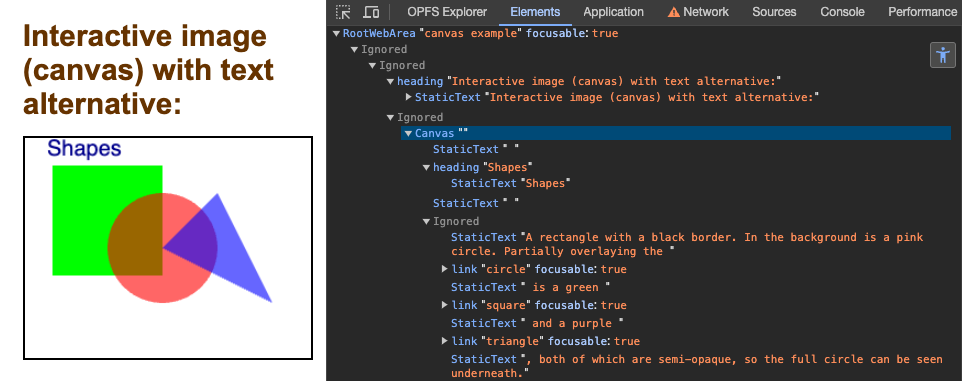
\includegraphics[width=\columnwidth]{canvas.png}
\caption{Inspecting the accessibility tree of an interactive canvas with text alternative.}
\label{fig:canvas}
\end{figure}

\subsection{The Accessibility Object Model}

Assistive technology such as screen readers use the browser's accessibility \textsc{api} to interact with web content. The underlying model of this \textsc{api} is the accessibility tree: a tree of accessibility objects that assistive technology can query for attributes and properties and perform actions on. Native \textsc{html} elements are implicitly mapped to accessibility \textsc{api}s. For example, an \texttt{img} element will automatically be mapped to an accessibility node with a role of \texttt{"image"} and a label based on the \texttt{alt} attribute (if present). Alternatively, \textsc{aria} allows developers to annotate elements to override the default role and semantic properties of an element, for example, to make a \texttt{div} act like a \texttt{button}.\footnote{Doing so is highly discouraged and developers should use a \texttt{button} directly.} Web developers shape and manipulate the accessibility tree primarily through \textsc{dom} properties such as \textsc{aria} attributes for \textsc{html}.\footnote{Accessible Rich Internet Applications (\textsc{wai}-\textsc{aria}) 1.3: \url{https://w3c.github.io/aria/}}

The Accessibility Object Model\footnote{Accessibility Object Model: \url{https://wicg.github.io/aom/spec/}} (\textsc{aom}) project aims to improve certain aspects of the user and developer experience concerning the interaction between Web pages and assistive technology. In particular, the project is concerned with improving the developer ability to express semantics for visual user interfaces which are not composed of elements, such as canvas-based user interfaces. At the time of this writing, the \textsc{aom} is still in an early draft stage. The original idea was to create \textit{virtual} nodes specifically for accessibility. See \autoref{lst:aom} for an example.

\begin{lstlisting}[language=JavaScript, style=ES6, label={lst:aom}, caption={The now retracted \texttt{AccessibleNode} \textsc{api} of the Accessibility Object Model.}]
// Conveying the semantics of a canvas-drawn table.
canvas.attachAccessibleRoot();
const table = canvas.accessibleRoot.append(new AccessibleNode());
table.role = 'table';
table.colCount = 10;
table.rowcount = 100;
const headerRow = table.append(new AccessibleNode());
headerRow.role = 'row';
// etc. 
\end{lstlisting}

One of the biggest concerns of this proposal was that any events fired on virtual nodes would immediately indication that the user is using assistive technology, which is private information that the user may not want to reveal. Adding a permission dialog might help if virtual nodes were only needed on a small number of specialized websites, but that would preclude their use in any widget library. To avoid privacy concerns, the currently feasible solution for custom-drawn \textsc{ui}s is to promote the use of true \textsc{dom} elements with \textsc{aria}, as described below.

\subsection{Hidden \textsc{dom} tree for canvas-rendered apps}

 The \textsc{dom} tree of fully canvas-rendered apps can, in the reductive case, consist of nothing more than a \texttt{canvas} element. This means that \textsc{dom}-based accessibility trees in browsers like Chrome\footnote{Accessibility tree in the Chrome browser: \url{https://developer.chrome.com/blog/full-accessibility-tree}} can't be populated. One approach for dealing with this is to recreate what's currently drawn onto the canvas in a hidden \textsc{dom} structure used exclusively by the browser to create the accessibility tree. Flutter\footnote{Flutter: \url{https://flutter.dev/}} is an industry framework that fully renders to a canvas to guarantee pixel perfection and platform consistency. The framework has a large number of default widgets that generate an accessibility tree automatically. For custom widgets, Flutter's \texttt{Semantics} class lets developers describe the meaning of their widgets, helping assistive technologies make sense of the widget content. For performance reasons, at the time of this writing, Flutter's accessibility is opt-in by default.
 
 The core idea in Flutter is to create an accessible \textsc{dom} structure that reflects what's currently displayed on the canvas (\autoref{fig:flutter}). This structure consists of an \texttt{flt-semantics-host} parent custom element that has any combination of \texttt{flt-semantics} and \texttt{flt-semantics-container} child elements that can themselves be nested. For example, what is represented in the accessibility tree as a button would not actually be a \texttt{button} in the \textsc{dom} structure. It's an \texttt{flt-semantics} element with an \texttt{aria-label} attribute, with the button's text as its value, and a \texttt{role} attribute with the value of \texttt{button}. It's made focusable by giving it a \texttt{tabindex} of \texttt{0}. This \texttt{flt-semantics} element is absolutely positioned to appear exactly where the corresponding button is painted on the canvas. As such, whenever the user scrolls, the positions need to be adjusted, which is \textsc{cpu}-intense. For text editing, Flutter has an \texttt{flt-text-editing-host} element that has either an \texttt{input} or a \texttt{textarea} as its child that it places with pixel precision onto the corresponding canvas area. Browser features such as autofill then work as expected. This feature is always enabled, independent of whether accessibility is enabled or not.

\begin{figure}[h]
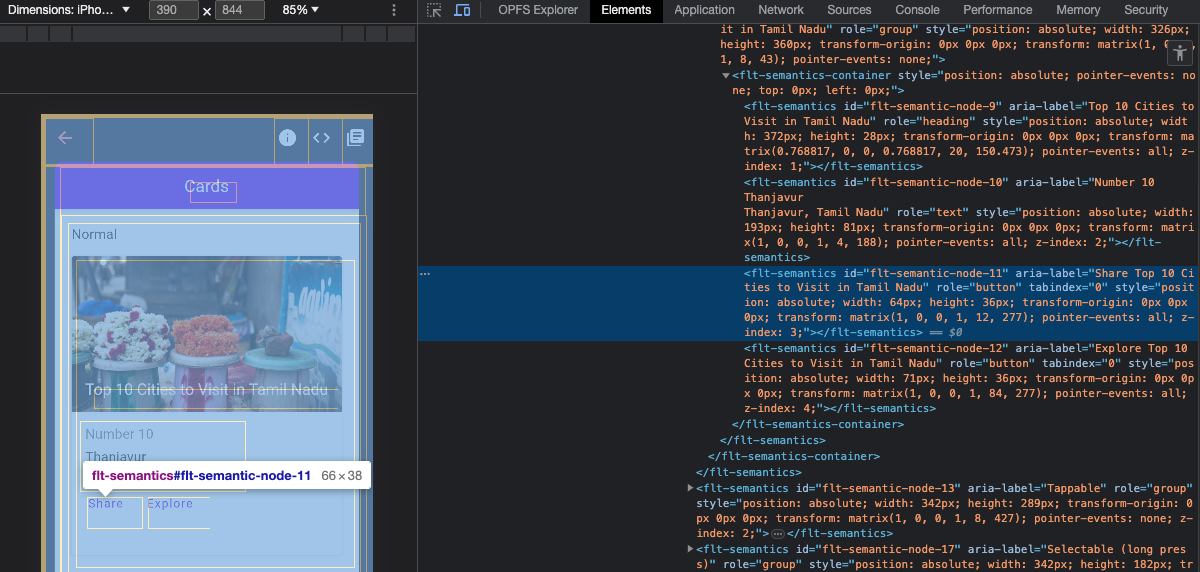
\includegraphics[width=\columnwidth]{flutter.png}
\caption{Flutter widget with hidden \textsc{dom} structure. (Source: \url{https://flutter-gallery-archive.web.app/#/demo/card})}
\label{fig:flutter}
\end{figure}

\subsection{Accessibility with AccessKit}

How could this approach be generalized for other frameworks that render to a canvas? Abstracting the solution of hidden \textsc{dom} structures is something the developers of an open-source project called AccessKit\footnote{AccessKit: \url{https://accesskit.dev/how-it-works/}} are working on: \textit{"The heart of AccessKit is a data schema that defines all the data required to render an accessible \textsc{ui} for screen readers and other assistive technologies. The schema represents a tree structure, in which each node or branch is either a single \textsc{ui} element, or an element cluster such as a window, pain, or document. Each node has an integer \textsc{id}, a role (\textit{e.g.}, button, edit, etc.) and a variety of optional attributes. The schema also defines actions that can be requested by assistive technologies, such as moving the keyboard focus, invoking a button, or selecting text"}. So-called platform adapters then implement the accessibility \textsc{api}s across various platforms. This cuts down significantly on development time when coding apps, as individual accessibility implementations will not need to be manually created for each platform. Currently, there are adapters for Windows, mac\textsc{OS}, and Unix, with plans for Android, i\textsc{OS}/tv\textsc{OS}, and Web (by creating a hidden \textsc{html dom}).

\section{Future directions---will \textsc{ai} save us?}

Rather than going from the original framework code bottom up to the to-be-generated accessibility tree, one could also imagine an \textsc{ai}-based approach. Here the \textsc{ai} would try \textit{ad hoc} to understand top-down what is currently painted onto the canvas, and translate that into an accessibility tree. Given enough training data, this could possibly work. However, the \textsc{ai} model would always be constrained to analyzing what it can currently "see" on the canvas. Anything outside of the canvas viewport, or anything outside of the viewport of a widget (like a long scrollable list box of hidden items), would be completely hidden from the \textsc{ai}. As such, this method seems problematic for some potential use cases. The processing power required to resolve in a timely manner may also be a limitation. Low-powered devices might already struggle with rendering the canvas application in the first place, and not have enough spare \textsc{cpu} cycles to run the \textsc{ai} on top. 

\section{Conclusions}

Opaque content has long existed on the Web, since the early days of Flash. Today, partial content like charts\footnote{Charts.js library: \url{https://www.chartjs.org/}} is rendered opaquely to a canvas, and some apps consist of nothing more than a sole canvas element (supported by loads of JavaScript and WebAssembly). Questions on the desirability of screen reader detection have been consistently explored, from heuristics that some apps use based on keyboard navigation patterns, to Flutter's opt-in button, to Flash's \texttt{flash.accessibility.Accessibility.active} property. Accessibility can't be an afterthought, and protecting the privacy of those dependent on assistive technologies is deeply rooted in the Web Platform Design Principles.\footnote{Web Platform Design Principles: \url{https://www.w3.org/TR/design-principles/#do-not-expose-use-of-assistive-tech}} On one hand, browser \textsc{api} designers need to ensure that their \textsc{api} requires user consent, before a developer can detect that an assistive technology is being used. Early versions of the well-intentioned \textsc{aom} did not respect this principle and were hence removed. On the other hand, the web platform must be accessible to people with disabilities, which, in the case of canvas-rendered apps or canvas-rendered content, can be challenging to impossible without knowing assistive technologies are in use. Ensuring the accessibility of opaque Web content has always been a challenge worth solving. Ironically, not using opaque Web content in the first place may be the simplest solution.
\end{document}
\endinput
